
\section{Serialization}
\label{serialization}

This section is about representing objects as a sequence of bytes. We will call this sequence \textit{stream}, its formal Type will be named $S$, the current stream will be named $s$. We will assume that there is an implicit conversion between fixed sized integers\footnote{As well as between fixed sized floating point numbers, because we define them to be IEEE-754 encoded 32-/64-bit sequences.} and streams. We also make use of a stream concatenation operator $\circ : S \times S → S$.

This section assumes, that all objects about to be serialized are already known. It further assumes, that their types and thus the values of the functions (i.e. baseTypeName, typeName, index, $\den{\_}$) explained below can be easily computed.


\subsection{Steps of the Serialization Process}

In general it is assumed that the serialization process is split into the following steps:
\begin{enumerate}
 \item All objects to be serialized are collected. This is usually done using the transitive closure of an initial set.
 
 \item The items are organized into their storage pools, i.e. the index function is calculated.
 
 \item The output stream is created as described below.
\end{enumerate}

\subsection{Reflection}
\todo{move to a suitable location; write a small chapter at the beginning as well}

so funktioniert die serialisierung des reflection pools (indices beschreiben den serialisierten typ, falls dieser unklar ist):

\begin{itemize}
 \item \den{REFL} = $\den{n}_{v64}\den{DECL_1} \circ \cdots \circ \den{DECL_n}$

 \item \den{DECL} = $\den{DESC}\den{name}\den{superName}\den{n}_{v64}\den{FIELD_1}\circ \cdots \circ \den{FIELD_n}$\footnote{Actually, only the serializable restrictions are taken from the DESC-part.}
 
 \item \den{HINT} = $\emptyset$
 
 \item \den{comment} = $\emptyset$
 
 \item \den{RESTRICTION} = $\emptyset$ iff. $id = \bot$
 \item \den{RESTRICTION} = $\den{id}_{v64}\den{ARG_1}_{string} \circ $ iff. $id \neq \bot$\footnote{eine tabelle mit IDs findet sich im Anhang}\todo{ref id-table}
 
 \item \den{FIELD} = \den{DESC}\den{TYPE}\den{name}
 
 \item \den{TYPE} = const ⇒ $id \circ \den{val}_{TYPE}$
 \item \den{TYPE} = $\varepsilon i. i \in [0,14] \wedge i = id(TYPE)$\todo{ref id-table}
 
 \item \den{T[i]} = $15 \circ \den{i}_{v64} \circ \den{T}$
 \item \den{T[f]} = $16 \circ \den{f.index}_{v64} \circ \den{T}$
 \item \den{T[]} = $17 \circ \den{T}$
 \item \den{\texttt{list}<T>} = $18 \circ \den{T}$
 \item \den{\texttt{set}<T>} = $19 \circ \den{T}$
 \item \den{\texttt{map}<T_1, \cdots, T_n>} = $20 \circ \den{n}_{v64} \circ \den{T_1} \circ \cdots \circ \den{T_n}$
 
 \item \den{T} = $\den{T.reflIndex + 21}_{v64}$

\end{itemize}



\subsection{Storage Pools}

\todo{folgendes layout eignet sich eigentlich besser}
\begin{verbatim}
v64 upperHalfCount
utf8[upperHalfCount][] significantStrings
[[reflectionPool]]
v64 lowerHalfSizeBytes
i8[lowerHalfSizeBytes] insignificantStrings

[[ordinary pools]]
\end{verbatim}
This allows for reading insignificant strings lazily.


\todo{sicherstellen, dass es verboten ist leere pools in eine datei zu schreiben}

This section contains the description of the high level file layout and gives meaning to the functions $baseTypeName: \mathcal{U} → S$, $typeName: \mathcal{U} → S$ and $index: \mathcal{U}\cup\{\textbf{string}\} → S$.

The basic idea behind the serialization format is to store the data grouped by type into storage pools. If objects are referred to from other objects, those references are usually given as integer, which is interpreted as index into the respective storage pool.

Because we will identify types by their name in human readable form, the first pool has to be the string pool. Because it is the first pool and the only pool, which stores objects of a built in type directly, it has a special layout. It starts with its size and is followed by exactly as many zero encoded utf8 strings. In a \gls{skill} inspired representation, this would look like: \footnote{Note that the utf8 type is not predefined in skill; it is used to distinguish between the serialization of a string typed field and the very string object.}
\begin{verbatim}
v64 size;
utf8[size] stringPool;
\end{verbatim}

Now, as we have the first pool, we can explain the \textit{index} function. All objects are stored concise pools, which basically can be seen as arrays of these objects. The index function returns the index of the objects, starting with the index 1\footnote{This is a bit unfortunate, because it may cause some bugs in language binding generators, but using the v64 encoding, it is important to save the 0 for the NULL pointer, as it is encoded with 1 byte instead of 9 bytes as it is the case for -1, which would be the most obvious alternative.} for the first object. The NULL pointer is represented by the index 0.

Because we want to allow for full reflection capabilities, but we do not want to force users to pay for the mechanism, if they do not require it, we spend a byte to indicate whether the required data is present or not. The data is stored as the last object in the string pool. In skill this part would be:
\begin{verbatim}
bool lastStringIsDefinition;
\end{verbatim}

The remaining part is the serialization of the remaining nonempty storage pools. First, these pools are sorted in ascending type order. Then the fields defined in the type stored in the pool are stored. Each pool keeps a start index, which allows for the reconstruction of the complete object. A short example shall illustrate the basic concept. It contains five types A,B,C,D and N. Each has a single field of type $\tau$ which is used to simplify the representation. The type information for the objects in the base type pool can be inferred from the data stored in the pools using the links between the base type pool and the subtype pools (The \gls{baseType} start index (BPSI) field of pools with a super type -- shown as arrows). For the sake of readability, the name, size and count fields are omitted in the picture.

\begin{figure}[h]
 

%NOTE: if this picture is used in a paper, colors have to be replaced by stippled lines
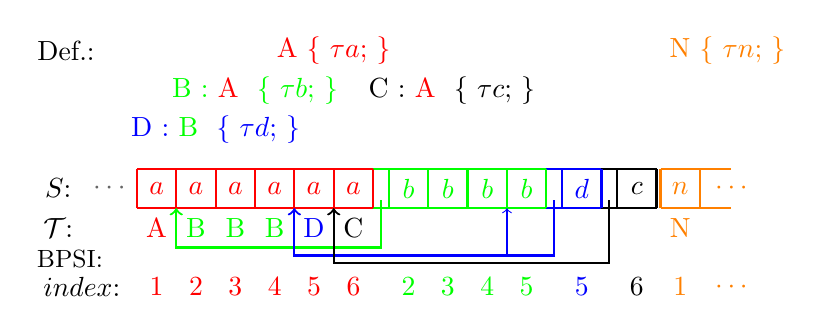
\begin{tikzpicture}
%labels
\node[draw=none] at (-1,0.25) {$S$:};
\node[draw=none] at (-1,-0.25) {$\mathcal{T}$:};
\node[draw=none] at (-0.7,-1) {$index$:};
\node[draw=none] at (-0.85,-0.65) {\small{BPSI}:};
\node[draw=none] at (-0.9,2) {Def.:};

%definitions
\node[red,draw=none] at (2.5,2) {A \{ $\tau a$; \} };
\node[green,draw=none] at (1.5,1.5) {B : {\color{red} A } \{ $\tau b$; \} };
\node[blue,draw=none] at (1,1) {D : {\color{green} B } \{ $\tau d$; \} };
\node[black,draw=none] at (4,1.5) {C : {\color{red} A } \{ $\tau c$; \} };

\node[orange,draw=none] at (7.5,2) {N \{ $\tau n$; \} };

%content
 \node[color=black!60,draw=none] at (-0.35,0.25) {$\cdots$};
 
 \node[red,draw=none] at (0.25,0.25) {${a}$};
 \node[red,draw=none] at (0.75,0.25) {${a}$};
 \node[red,draw=none] at (1.25,0.25) {${a}$};
 \node[red,draw=none] at (1.75,0.25) {${a}$};
 \node[red,draw=none] at (2.25,0.25) {${a}$};
 \node[red,draw=none] at (2.75,0.25) {${a}$};
 
 \node[green,draw=none] at (3.45,0.25) {$b$};
 \node[green,draw=none] at (3.95,0.25) {${b}$};
 \node[green,draw=none] at (4.45,0.25) {${b}$};
 \node[green,draw=none] at (4.95,0.25) {${b}$};
 
 \node[blue,draw=none] at (5.65,0.25) {${d}$};
 
 \node[black,draw=none] at (6.35,0.25) {${c}$};
 
 \node[orange,draw=none] at (6.9,0.25) {${n}$};
 \node[orange,draw=none] at (7.55,0.25) {$\cdots$};
 
%base pool index
 
 \node[red,draw=none] at (0.25,-1) {1};
 \node[red,draw=none] at (0.75,-1) {2};
 \node[red,draw=none] at (1.25,-1) {3};
 \node[red,draw=none] at (1.75,-1) {4};
 \node[red,draw=none] at (2.25,-1) {5};
 \node[red,draw=none] at (2.75,-1) {6};
 
 \node[green,draw=none] at (3.45,-1) {2};
 \node[green,draw=none] at (3.95,-1) {3};
 \node[green,draw=none] at (4.45,-1) {4};
 \node[green,draw=none] at (4.95,-1) {5};
 
 \node[blue,draw=none] at (5.65,-1) {5};
 
 \node[black,draw=none] at (6.35,-1) {6};
 
 \node[orange,draw=none] at (6.9,-1) {1};
 \node[orange,draw=none] at (7.55,-1) {$\cdots$};
 
%base pool types
 \node[red,draw=none] at (0.25,-0.25) {A};
 \node[green,draw=none] at (0.75,-0.25) {B};
 \node[green,draw=none] at (1.25,-0.25) {B};
 \node[green,draw=none] at (1.75,-0.25) {B};
 \node[blue,draw=none] at (2.25,-0.25) {D};
 
 \node[black,draw=none] at (2.75,-0.25) {C};
 
 \node[orange,draw=none] at (6.9,-0.25) {N};

%frames
 \draw[shift={(0.15,0)},thick,orange] (6.4999,0) grid [step=0.5] (7.4,0.5);

 \draw[shift={(0.6,0)},thick,black] (5.3,0) grid [step=0.5] (6,0.5);
 \draw[shift={(0.4,0)},thick,blue] (4.8,0) grid [step=0.5] (5.5,0.5);
 \draw[shift={(0.2,0)},thick,green] (2.8,0) grid [step=0.5] (5,0.5);
 \draw[thick,red] (0,0) grid [step=0.5] (3,0.5);
 
%base type indices
 \draw[thick,green,->] (3.1,0.1) -- (3.1,-0.5) -- (0.5,-0.5) -- (0.5,0);
 \draw[thick,blue,->] (5.3,0.1) -- (5.3,-0.6) -- (2,-0.6) -- (2,0);
 \draw[blue,->] (5.3,0.1) -- (5.3,-0.6) -- (4.7,-0.6) -- (4.7,0);
 \draw[thick,black,->] (6,0.1) -- (6,-0.7) -- (2.5,-0.7) -- (2.5,0);
\end{tikzpicture}
\caption{The serialization scheme used to store objects into pools.}
\end{figure}

Note, that the pool of D comes in front of the pool of C, because it is smaller according to the type order.

This leads to the serialization of a pool as:
\begin{verbatim}
v64 poolName
option(v64 basePoolStartIndex; iff has superType)
v64 sizeCount
v64 sizeBytes
T[sizeCount] elements
\end{verbatim}

The poolName is an index into the string pool and points to the type name stored in the pool.

The sizeCount contains the number of elements in the pool. This is required in order to move objects of an unknown subtype. It does also simplify the deserialization process.

The basePoolStartIndex is the index of the first element in the base types pool.



A concise description of the file layout could look like this:
\begin{verbatim}
v64 size
utf8[size] stringPool
[[TODO ...]]

while(next!=EOF){
  v64 poolName
  option(v64 basePoolStartIndex; iff has superType)
  v64 sizeCount
  v64 sizeBytes
  [[ T[sizeCount] elements ]]
}
\end{verbatim}

An interesting observation about this encoding is, that the shortest legal file consists of two bytes, which are both zero. Although the encoding makes use of various invariants it provides some means of error detection, as explained in the appendix.

\subsection{Pool Elements}

Let $\den{\_}:\mathcal{T} → S$ be the translation function, which serializes a field of an object into a stream. The serialization of an objects takes places by serializing all its fields in canonical field order into the stream. In this section, we assume that the three functions defined in the last section are implicitly converted to streams using the v64 encoding. We assume further, that compound types provide a function $size: \mathcal{T} → \mathcal{I}$, which returns the number of elements stored in a given field.
Let $f$ be a field of type $t$, then $\den{f}$ is defined as\footnote{We will use C-Style hexadecimal integer literals for integers in streams.}
\begin{itemize}
 %null
 \item $\forall t \in \mathcal{U}\cup\{\textbf{string}\}. \den{\texttt{NULL}} = \texttt{0x00}$
 %pooled objects
 \item $\forall t \in \mathcal{U}\cup\{\textbf{string}\}. \den{f} = index(f)$
 
 %annotation -> * (v64 baseTypeName!!, v64index)
 \item $t=\textbf{annotation} \implies \den{\texttt{NULL}} = \texttt{0x00} \circ 0x00$\footnote{the first value is not important and may change in the future; it results from the encoding requiring a type for the null pointer.}
 \item $t=\textbf{annotation} \implies \den{f} = baseTypeName(f) \circ index(t)$ \todo{hier eignet sich die type ID deutlich besser!}
 
 %bool
 \item $t=\textbf{bool} \implies \den{\top} = \texttt{0xFF} \wedge \den{\bot} = \texttt{0x00}$
 
 %fixed int
 \item $\forall t \in \mathcal{I}\setminus\{\textbf{v64}\}. \den{f} = f$
 
 %v64
 \item $\forall t \in \{\textbf{v64}\}. \den{f} = encode(f)$\footnote{With encode as defined in listing \ref{v64enc}.}
 
 %fixed float
 \item $\forall t \in \{\textbf{f32},\textbf{f64}\}. \den{f} = f$\footnote{Assuming the float to be IEEE-754 encoded, which allows for an implicit bit-wise conversion to fixed sized integer.}
 
 %fixed and dependent arrays
 \item $\forall g \in \mathcal{B}, n \in \mathbb{N}^+. t = g\texttt{[}n\texttt{]} \implies \den{f} = \den{f_0} \circ \cdots \circ \den{f_{n-1}}$
 
 \item $\forall g \in \mathcal{B}, s \in \mathcal{I}, \texttt{s size}$\footnote{As stated above, size must be a field of the same declaration as f.} $. t = g\texttt{[size]} \wedge \texttt{size} \geq 0 \implies \den{f} = \den{f_0} \circ \cdots \circ \den{f_{\texttt{size}-1}}$\footnote{Note that this is the only case where the encoded field does not append anything to the stream.}
 
 %variable array, list and set
 \item $\forall g \in \mathcal{B}, n = size(f). t \in \{g\texttt{[]}, \texttt{set<}g\texttt{>}, \texttt{list<}g\texttt{>}\} \implies \den{f} = \den{n} \circ \den{f_0} \circ \cdots \circ \den{f_{n-1}}$
 
 %map
 \item Maps are serialized from left to right by serializing the keyset and amending each key with the map structure which it points to. In case of Maps with two types, this is equal to a list of key value tuples.
 A field of type \verb/map<T,U,V>/ is serialized using a schema $ \den{size(f)} \circ \den{f.t_1} \circ \den{size(f[t_1])} \circ \den{f[t_1].u_1} \circ \den{f[t_1][u_1]} \circ \den{f[t_1].u_2} \circ \cdots \circ \den{size(f[t_2])} \circ \cdots \circ \den{f[t_n][u_m]}$
\end{itemize}




\section{Deserialization}

Deserialization is mostly straight forward.

The general strategy is:
\begin{itemize}
 \item the string pool is deserialized and a map from index to strings is created.
 \item the type structure is reconstructed while the pools are copied into memory
 \item objects are reconstructed
\end{itemize}
